\documentclass[12pt]{article}
\usepackage[margin=1in]{geometry}
\usepackage{float}
\usepackage[T1]{fontenc}
\usepackage{listings}
\usepackage{graphicx}
\usepackage{placeins}
\usepackage[nottoc]{tocbibind} %Adds "References" to the table of contents
\usepackage{graphicx}
\usepackage{listings}

\newlength\tindent
\setlength{\tindent}{\parindent}
\setlength{\parindent}{0pt}
\renewcommand{\indent}{\hspace*{\tindent}}

\lstset{
	frame=tb,
	showstringspaces=false,
	columns=flexible,
	breaklines=true,
	breakatwhitespace=true
}

\begin{document}
\pagenumbering{gobble}
\begin{titlepage}
   \vspace*{\stretch{1.0}}
   \begin{center}
      \textsc{\Huge プログラミング実験第三}\\ [1cm]
      \textsc{\Huge TinyJavaScript コンパイラの作り直し}\\ [2cm]
      \large\textit{\huge 1311216}\\
      \large\textit{\huge Rathore Amogh\\}
      \large\textit{\huge 岩崎研究室\\}
   \end{center}
   \vspace*{\stretch{2.0}}
\end{titlepage}


\tableofcontents

\newpage
\pagenumbering{arabic}

\section{はじめに}
\subsection{背景}
TinyJavaScript は JavaScript の一部機能を制限んしたサブセットのことである\cite{jscompiler}。TinyJavaScriptの元のコンパイラは Mozilla の SpiderMonkey Parser API \cite{spidermonkey}を使用していた。しかし、SpiderMonkey Parser は絶えてしまって、TinyJavaScript のコンパイラの開発も続けられなくなった。だから、TinyJavaScript コンパイラを新しいパーサを使用して作りなおす必要が出てきた。このレポートは TinyJavaScript コンパイラを Node JS で作る実験について述べる。

\subsection{実験の目的}
この実験ではTinyJavaScriptのコンパイラをNodeJSとEsprima (ECMAScript Parsing Infrastructure for Multipurpose Analysis) \cite{esprima}を使用して実装する。それで、コンパイラの作り方と構造について学習する。最後に、実験で作った新しいコンパイラとTinyJavaScriptの\cite{jscompiler}で述べてるコンパイラの比較を行う。

\subsection{実装の方針}
実装にはEsprimaというECMAScript\cite{ecmascript} Parserを使用する。JavaScriptはECMAScriptのdialectであるので、ECMAScriptのパーサはJavaScriptの構文に対して正しくパーシングをされる。参考のため\cite{jscompiler}で述べてるTinyJavaScript Compilerの実装を使う。もう少し具体的に言うと、Esprimaを使ってTinyJavaScriptのソースコードを抽象構文木に変換する。それから、抽象構文木をトラバースしてSSJSVM(これについて後で述べる)の命令列を生成する。

\section{TinyJavaScript と SSJSVM}
\subsection{TinyJavaScript}
TinyJavaScriptはJavaScriptの以下の機能をサポートしない \cite{jscompiler}
\begin{itemize}
\item with 文
\item delete 文
\item グローバル変数宣言時の var の省略
\item for in 文
\item switch 文
\item 名前付きの関数定義
\end{itemize}

\cite{jscompiler}よりTinyJavaScriptの文法規則が図\ref{grammarFig}通りである。
\begin{figure}
\centering
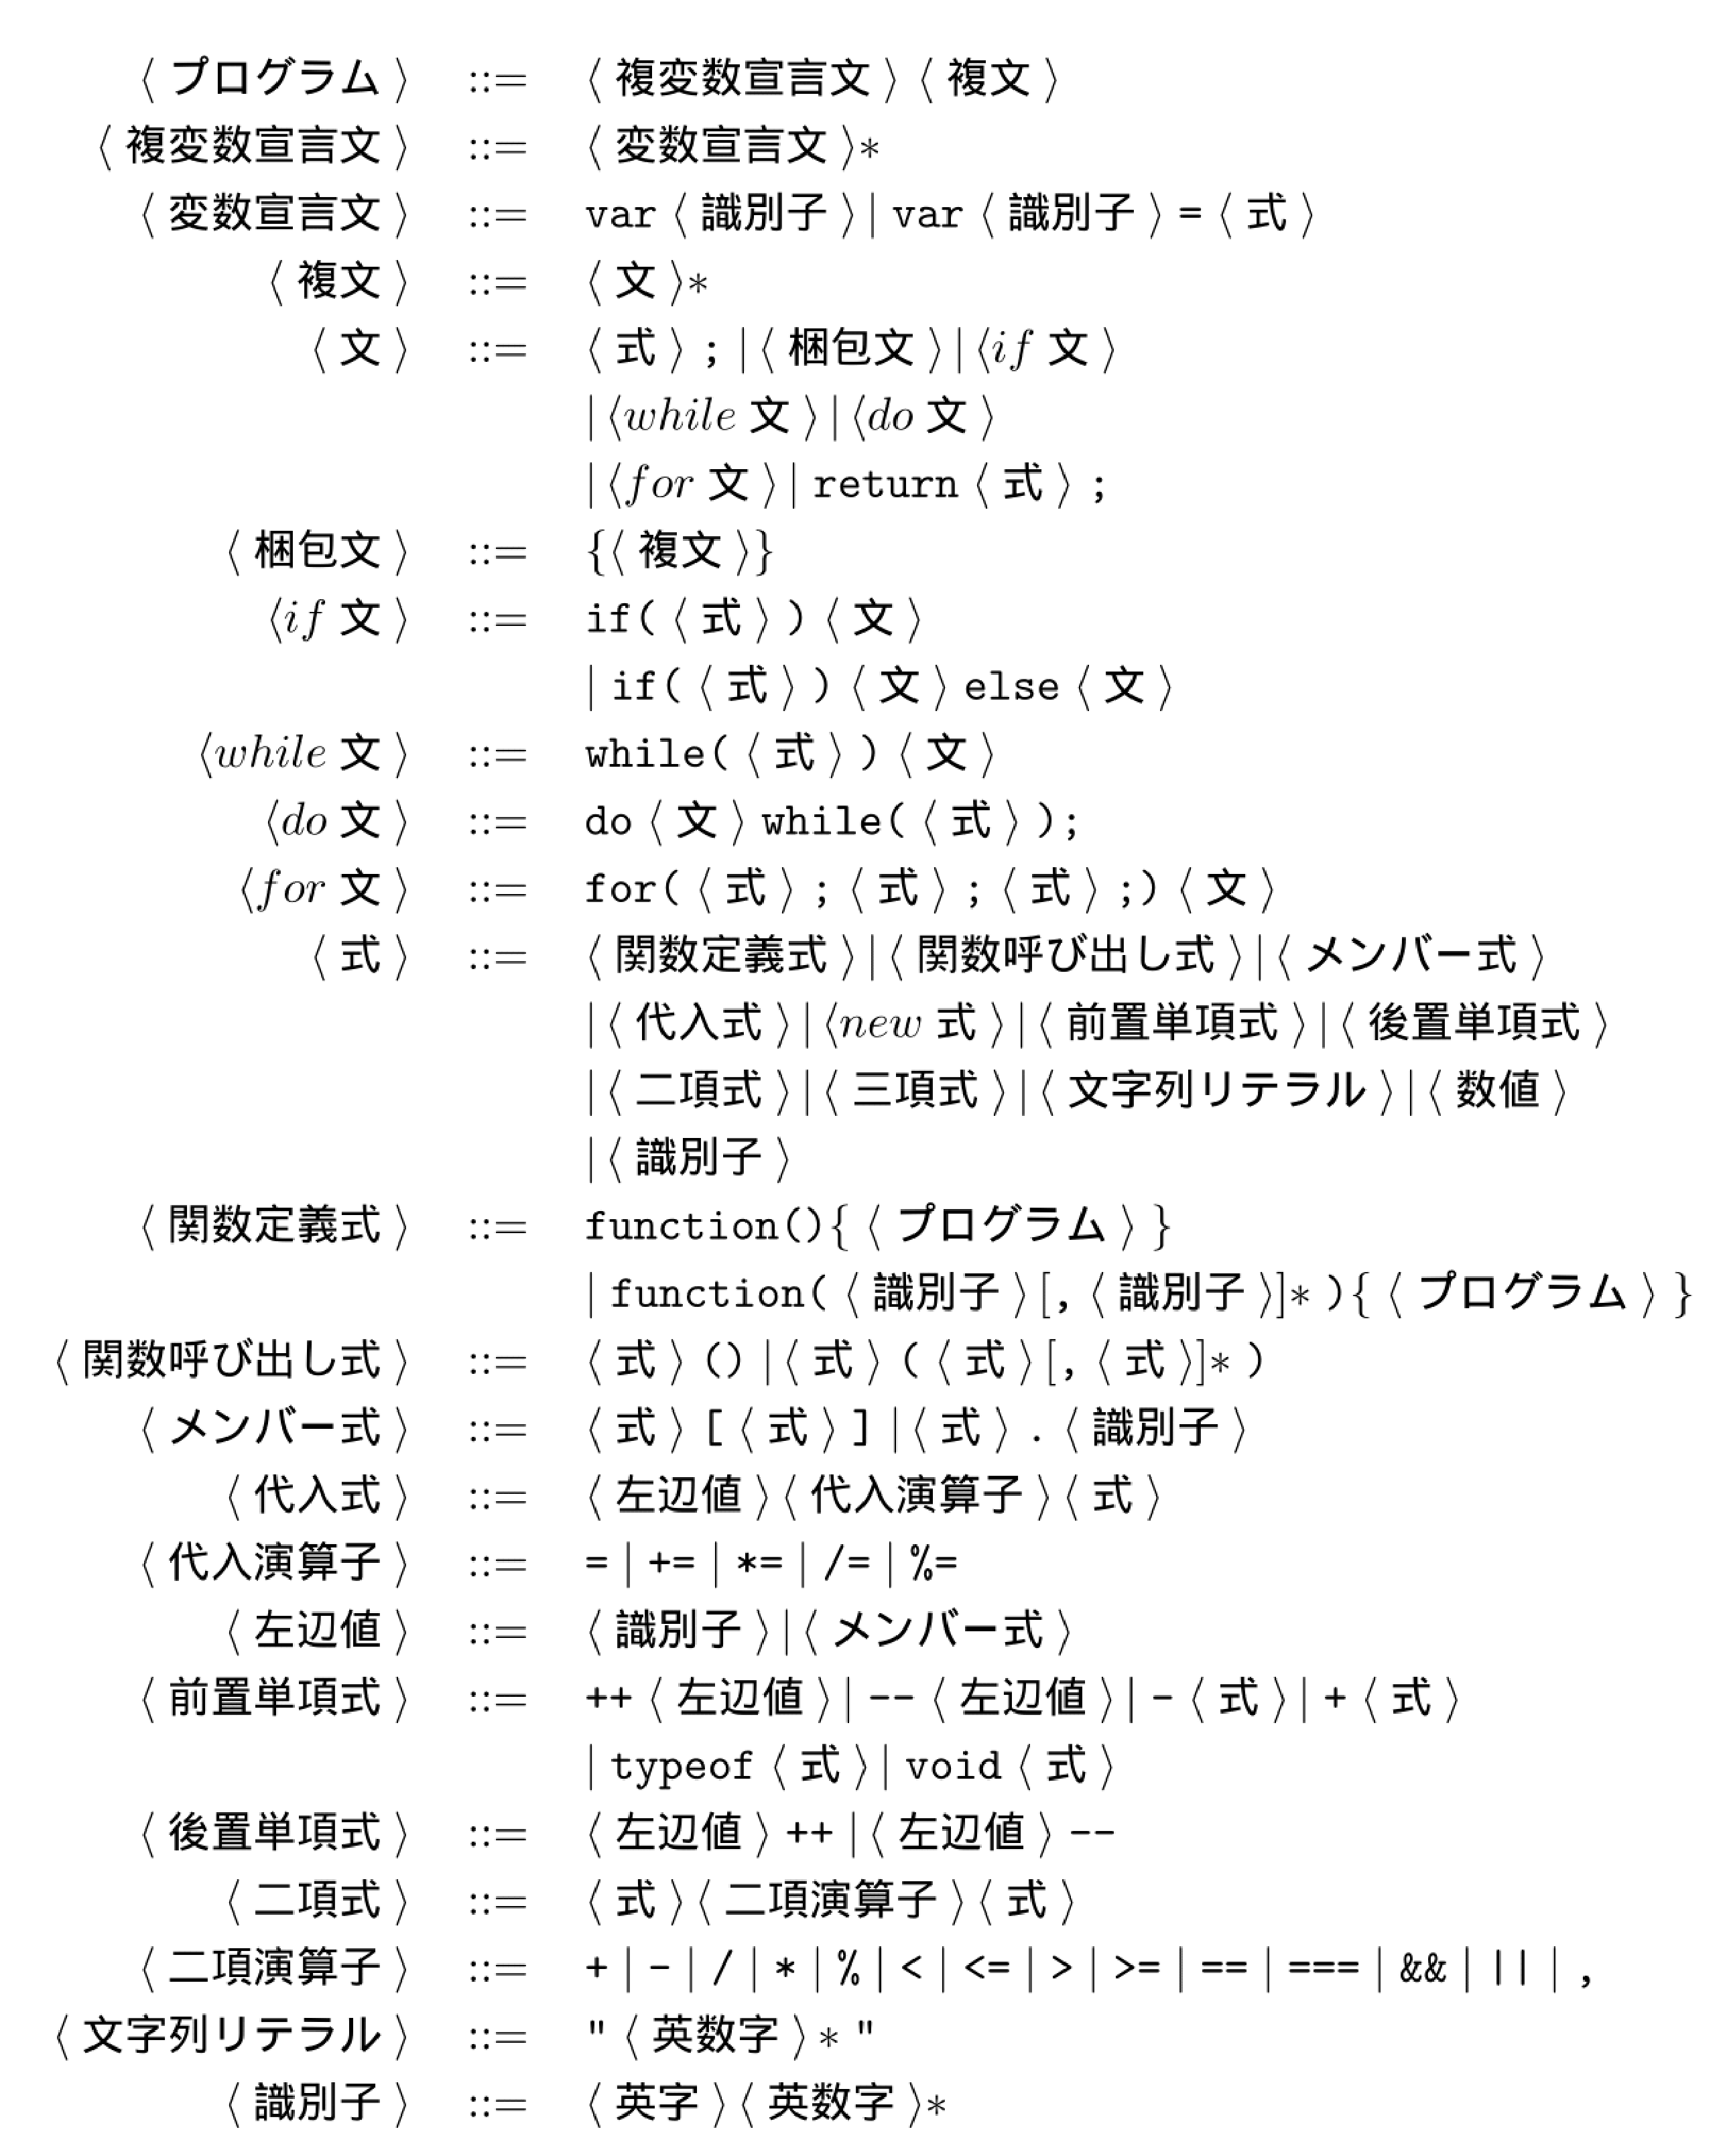
\includegraphics[scale=0.41]{grammar.eps}
\caption{TinyJavaScriptの文法規則}
\label{grammarFig}
\end{figure}
\FloatBarrier

\subsection{SSJSVM}
SSJSVM は Server-side JavaScript Virtual Machine の略称である。すなわち、サーバで動くJavaScriptの仮想機械のことである。本実験では、TinyJavaScriptのソースコードをSSJSVMの命令列に変換するコンパイラを作る。

\section{パーサの選び方}
実験の目的はTinyJavaScriptのコンパイラを新しいパーサ(SpiderMonkey 1.6でないパーサ)を使用して作るということである。だから、プログラミングを始める前にパーサを選ぶ必要がある。以下の特徴を持つパーサを使いたい。

\begin{enumerate}
\item ECMAScript の新しいバージョンをサポートする
\item 構文解析を正しくやってくれる
\item 使いやすい
\item ドキュメントとサポートがいい
\end{enumerate}

いろいろ調べた結果、2つの案が出てきた。

\begin{itemize}
\item ECMAScriptの文法を揃えてANTLR\cite{antlr} (ANother Tool for Language Recognition)を使ってパーサを生成する
\item Esprima を使う
\end{itemize}

ANTLRを使用するとANTLR用の文法が必要となる。その文法はいろいろなソースがインターネットで提供してるが、オフィシャルではないので正しさは保証できない。あとドキュメントなども全然提供されてなくて、使いにくいと判断した。ところで、Esprimaはとてもアクチブなプロジェクトであって、投稿者が多い。だから、最後にEsprimaを使うと決める。

\section{Esprima}
\subsection{特徴}
Esprima \cite{esprima}はJavaScriptで書かれてるECMAScriptのパーシングインフラストラクチャである。Esprimaの主な特徴は以下のとおりである\cite{esprima}。
\subsection{例}
Esprimaには「parse」メソッドがあって、そのメソッドにソースコードをストリングで渡すと抽象構文木がJSオブジェクトで返される。

\begin{lstlisting}
var a = 2;
\end{lstlisting}
\FloatBarrier

上の変数宣言のコードの抽象構文木オブジェクトのJSONは以下のようである。

\begin{lstlisting}
	{
	    "type": "Program",
	    "body": [
	        {
	            "type": "VariableDeclaration",
	            "declarations": [
	                {
	                    "type": "VariableDeclarator",
	                    "id": {
	                        "type": "Identifier",
	                        "name": "a"
	                    },
	                    "init": {
	                        "type": "Literal",
	                        "value": 2,
	                        "raw": "2"
	                    }
	                }
	            ],
	            "kind": "var"
	        }
	    ],
	    "sourceType": "script"
	}
\end{lstlisting}
\FloatBarrier

\begin{lstlisting}
var a = ["amogh", "rathore", 21];
\end{lstlisting}
\FloatBarrier

配列なら以下のようになる。

\begin{lstlisting}
	{
	    "type": "Program",
	    "body": [
	        {
	            "type": "VariableDeclaration",
	            "declarations": [
	                {
	                    "type": "VariableDeclarator",
	                    "id": {
	                        "type": "Identifier",
	                        "name": "a"
	                    },
	                    "init": {
	                        "type": "ArrayExpression",
	                        "elements": [
	                            {
	                                "type": "Literal",
	                                "value": "amogh",
	                                "raw": "\"amogh\""
	                            },
	                            {
	                                "type": "Literal",
	                                "value": "rathore",
	                                "raw": "\"rathore\""
	                            },
	                            {
	                                "type": "Literal",
	                                "value": 21,
	                                "raw": "21"
	                            }
	                        ]
	                    }
	                }
	            ],
	            "kind": "var"
	        }
	    ],
	    "sourceType": "script"
	}
\end{lstlisting}
\FloatBarrier

上からわかるように、各構文は「type」というプロパーティが付いている。そのプロパーティから構文の種類(BNFの非終端記号と一緒)がわかる。

\begin{itemize}
\item ECMAScript 6 (ECMA-262 \cite{ecmascript}) 全体をサポート
\item Estree プロジェクトの標準を対応する構文木フォーマット
\item よくテストされたパーサ \cite{esprimaTests}
\item オープンソース \cite{esprimaGitHub}
\end{itemize}

\section{コンパイラの設計}
本実験で作るコンパイラは、ソースコードを3つの段階で仮想機械の命令列に変換する。その段階は以下の通りである。

\begin{figure}
\centering
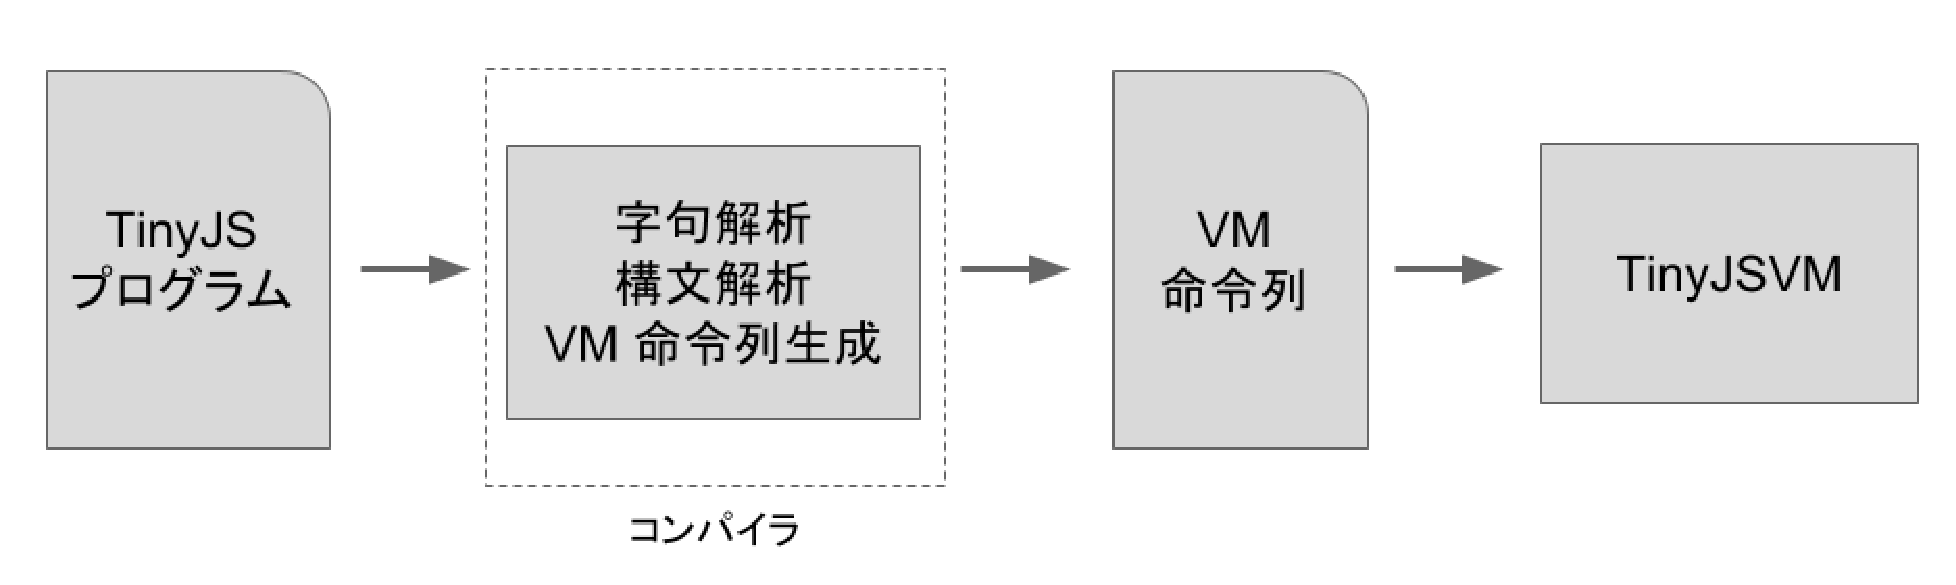
\includegraphics[scale=0.5]{process.eps}
\caption{コンパイルの3つの段階}
\end{figure}
\FloatBarrier

\begin{enumerate}
\item ソースコードの字句解析を行う
\item 字句列から抽象構文木を生成する
\item 抽象構文木を仮想機械の命令列に変換する
\end{enumerate}

本実験で使うEsprimaパーサは段階1と段階2の処理を行ってくれる。Esprimaは抽象構文木をJSオブジェクトにして返す。

\section{コンパイラの実装}
この説でコンパイラの実装を述べる。コンパイラは各構文に対して別の変換を行うので、各構文に対しての処理をこれから述べる。

\subsection{Literalタイプ}
EsprimaのLiteralタイプは数値、真偽値や undefined などの定数、文字列、正規表現を含んでいる。

\subsubsection{数値}
数値の命令列を生成するために、まずは整数かどうかを調べる。なぜなら、SSJSVMで整数と浮動小数点数に対して別の命令が存在するから。コンパイラはNodeJSで書くので、JSのNumber.isSafeInteger()メソッドを使って、整数かどうかを判断する。整数ならfixnum、整数でないならnumberという命令を使う。\\

例:var a = 3; の'2'のところは以下のようになる
\begin{lstlisting}
...
fixnum 2 2
...
\end{lstlisting}
\FloatBarrier

整数でない場合は、すなわち var a = 2.5; の場合
\begin{lstlisting}
...
number 2 2.5
...
\end{lstlisting}
\FloatBarrier

のようになる。

\subsubsection{真偽値や undefined などの定数}
この場合は、SSJSVMの「specconst」という命令を使う。specconst命令は引数で定数を以下のように受け取る。\\

\begin{table}[h]
\centering
\begin{tabular}{|c|c|}
	\hline
	定数 & SSJSVMで使う引数 \\
	\hline
	true & true \\
	false & false \\
	null & null \\
	undefined & undefined \\
	\hline
\end{tabular}
\end{table}

例:var a = true; は以下のようになる\\

\begin{lstlisting}
...
specconst 2 true
...
\end{lstlisting}

\subsubsection{文字列}
文字列の場合、SSJSVMの「string」命令を使う。

例:var a = "amogh";\\

\begin{lstlisting}
...
string 2 "amogh"
...
\end{lstlisting}

\subsubsection{正規表現}
この場合、SSJSVMの「regexp」命令を使う。JavaScriptの正規表現のフラッグを整数のビットに保持して渡す。

例:var a = /d(b+)d/g; の場合\\

\begin{lstlisting}
...
regexp 2 1 "d(b+)d"
...
\end{lstlisting}

のようになる。ここで、2はレジスターで、1は正規表現のフラッグを表す。1の意味はフラッグgが立ててることを表す。

\subsection{バイナリ式 (BinaryExpressionタイプ)}
バイナリ式の場合、まずは演算子の左辺と右辺を評価して、2つのレジスタに保持する。次に、2つのレジスタの値をオペランドにして、演算子に対応する適当な命令を使う。演算子と命令は以下の通りである。

\begin{table}[h]
\centering
\begin{tabular}{|c|c|}
	\hline
	演算子 & 命令 \\
	\hline
	< & lessthan \\
	<= & lessthanequal \\
	> & greaterthan \\
	>= & greaterthanequal \\
	== & JSなので複雑な手順を使わないといけないが、equal命令を使う \\
	=== & eq \\
	+ & add \\
	- & sub \\
	$\star$ & mul \\
	/ & div \\
	\% & mod \\
	\& & bitand \\
	| & bitor \\
	< < & leftshift \\
	> > & rightshift \\
	> > > & unsignedrightshift \\
	\hline
\end{tabular}
\end{table}
\FloatBarrier

例: 5 + 10; の場合以下のようになる\\

\begin{lstlisting}
...
fixnum 3 1
fixnum 4 2
add 2 3 4
...
\end{lstlisting}
\FloatBarrier

\subsection{変数 (Identifierタイプ)}
変数の環境をまず求める。それは、localかglobalかargのいずれかである。環境を求めたあと命令を以下のように決める。

\begin{table}[h]
\centering
\begin{tabular}{|c|c|}
	\hline
	環境 & 命令 \\
	\hline
 	local & getlocal \\
	global & getglobal \\
	arg & getarg \\
	\hline
\end{tabular}
\end{table}

\subsection{代入 (AssignmentExpressionタイプ)}
まずは、左辺の種類を求める。すなわち、変数かプロパーティかを判断する。

\subsubsection{変数の場合 (左辺はIdentifierタイプ)}
まずは変数の環境を求める。次に、環境によって、以下のように命令を決める。

\begin{table}[h]
\centering
\begin{tabular}{|c|c|}
	\hline
	環境 & 命令 \\
	\hline
 	local & setlocal \\
	global & setglobal \\
	arg & setarg \\
	\hline
\end{tabular}
\end{table}
\FloatBarrier

例:a = "some string"; の場合\\

\begin{lstlisting}
...
string 2 "some string"
string 5 "a"
setglobal 5 2
...
\end{lstlisting}
\FloatBarrier

\subsubsection{プロパーティの場合 (左辺はMemberExpressionタイプ)}
ここはまた2つ種類がある。左辺は . を使った代入と、左辺は [ ] を使った代入。\\

. を使った代入だとまずは . の左辺の変数(Identifier)をコンパイルしてレジスタ t1 に保持する。その後、= の右辺の式をコンパイルしてレジスタ t2 に保持する。それから、. の右辺のプロパーティに対してstring命令を使ってそれをレジスタ t3 に保持する。最後に setprop t1 t2 t3 命令を使ってプロパーティに代入する。\\

例:a.prop = 10; の場合は以下のようになる

\begin{lstlisting}
...
string 7 "a"
getglobal 3 7
fixnum 2 10
string 5 "prop"
setprop 3 5 2
...
\end{lstlisting}
\FloatBarrier
\hfill \break
[ ] を使った場合は、[ ]の左辺の変数をコンパイルしてレジスタt1に保持する。[ ]の中身をコンパイルしてレジスタt3に保持する。= の右辺をコンパイルしてレジスタt2に保持する。最後に、setprop t1 t2 t3 命令を使ってプロパーティに代入する。

\subsection{ConditionalExpressionタイプ}
e1?e2:e3 を考える。2つのラベルL1とL2を用意する。まずは、e1 をコンパイルして結果をレジスタ t に保持する。次に、t が false ならL1にジャンプする命令を生成する。その後はe2をコンパイルして、ラベルL2にジャンプする命令を生成する。それは、tがtrueならe3に行かないからである。それから、ラベルL1をつけて、e3をコンパイルする。最後にラベルL2をつける。

例: a > b ? 3 : 5; の場合は以下のようになる。\\

\begin{lstlisting}
...
string 6 "a"
getglobal 4 6
string 7 "b"
getglobal 5 7
lessthan 3 5 4
jumpfalse 3 3
fixnum 2 3
jump 2
fixnum 2 5
...
\end{lstlisting}

\subsection{if else 文 (IfStatementタイプ)}
これもConditionalExpressionと同様である。

\subsection{while文 (WhileStatementタイプ)}
while文をコンパイルするために、まずはラベルL1へジャンプする命令を生成する。次に、ラベルL2をつけて、while文の身体をコンパイルする。それから、ラベルL1をつけて、while文のテストをコンパイルして、テストの結果をレジスタtに保持する。最後に、tがtrueなら、L2へジャンプする命令を生成する。そうすると、先にテストが実行されて、結果がtrue場合、中身が実行されてまたテストが実行されるようになる。

例: while(a > b) b = b+1;\\

\begin{lstlisting}
...
jump 7
string 8 "b"
getglobal 6 8
fixnum 7 1
add 2 6 7
string 9 "b"
setglobal 9 2
string 12 "a"
getglobal 10 12
string 13 "b"
getglobal 11 13
lessthan 3 11 10
jumptrue 3 -11
...
\end{lstlisting}

\subsection{do while (DoWhileStatementタイプ)}
これはwhile文と同様な実装である。まずはラベルL1をつけて、中身をコンパイルする。次に、テストをコンパイルして、結果がtrueならL1へジャンプする。

例:do b = b+1; while(a > b)\\

\begin{lstlisting}
...
string 8 "b"
getglobal 6 8
fixnum 7 1
add 2 6 7
string 9 "b"
setglobal 9 2
string 12 "a"
getglobal 10 12
string 13 "b"
getglobal 11 13
lessthan 3 11 10
jumptrue 3 -11
...
\end{lstlisting}

\subsection{for文 (ForStatementタイプ)}
for文を実装するために、まずはfor文の初期化の部分をコンパイルする。次に、ラベルL1へジャンプする命令を生成する。その後、ラベルL2をつけて、for文の中身をコンパイルして、for文のアップデート文をコンパイルする。それから、ラベルL1をつけて、テストの部分をコンパイルする。最後に、テストの結果がtrueならば、ラベルL2へジャンプする。そうすると、for文の初期化の部分が先に一回実行されて、次にテストが実行される。テストの結果がtrueなら、中身とアップデートが順に実行される。それからまたテストが実行されるようになる。

例:for(var i=0; i<10; i=i+1) b = b+1;\\

\begin{lstlisting}
...
fixnum 3 0
string 4 "i"
setglobal 4 3
jump 13
string 9 "b"
getglobal 7 9
fixnum 8 1
add 2 7 8
string 10 "b"
setglobal 10 2
string 15 "i"
getglobal 13 15
fixnum 14 1
add 3 13 14
string 16 "i"
setglobal 16 3
string 19 "i"
getglobal 17 19
fixnum 18 10
lessthan 3 17 18
jumptrue 3 -16
...
\end{lstlisting}

\subsection{リターン文 (ReturnStatementタイプ)}
リターンされた値をTinyJavaScriptで「a」というレジスターに保持するべきである。だから、リターン文の身体をコンパイルして、結果をあるレジスターtに保持する。それから命令setaを使ってtの値をaにセットする。最後に、SSJSVMのret命令を使ってリターン文のコンパイルを完了する。

例:var fun = function(){	return 10; }\\

\begin{lstlisting}
...
fixnum 3 10
seta 3
ret
...
\end{lstlisting}

\subsection{レシーバのある関数呼び出し (calleeプロパーティのタイプがMemberExpressionタイプであるCallExpressionタイプ)}
メソッドの呼び出しを実装するために、まずはレシーバをコンパイルする。Esprimaでそれはcallee.objectプロパーティに入ってる。それから、レシーバのメソッドをstring命令とgetprop命令を使ってフェッチする。それから、引数をそれぞれコンパイルして結果をレジスーt1~tnに保持する。それから、move命令を使って引数の結果をすべてスタックフレームにロードする。テールフラッグが立ててれば、tailsend命令を使う。立ててなければ、レジスターウインドウの大きさを計算してsetflコマンドを使って新しいフレームリンクを作る。最後に、結果をリターンするためにレジスターaに保持する。

例(tailflagが付いていない): a.x(x1, x2); \\

\begin{lstlisting}
...
setfl 17
string 8 "a"
getglobal 5 8
string 4 "x"
getprop 3 5 4
string 9 "x1"
getglobal 6 9
string 10 "x2"
getglobal 7 10
move 15 5
move 16 6
move 17 7
send 3 2
setfl 17
geta 2
seta 2
ret
...
\end{lstlisting}

\subsection{レシーバのない関数呼び出し (calleeプロパーティのタイプがMemberExpressionタイプでないCallExpressionタイプ)}
まずは関数名をコンパイルする。そのあと、すべての引数を順にコンパイルする。それから、すべての引数をコンパイルした結果をスタックフレームにロードする。テールフラッグが立てれば、tailsend命令を使う。立ててなければ、レジスターウインドウの大きさを計算してsetflコマンドを使って新しいフレームリンクを作る。最後に、結果をリターンするためにレジスターaに保持する。

\subsection{単項式 (UnaryExpressionタイプ)}
命令を以下のように決める。

\begin{table}[h]
\centering
\begin{tabular}{|c|c|}
	\hline
	オペレタ & オペランド \\
	\hline
	! & not \\
	- & mul で -1と掛け算する \\
	typeof & typeof \\
	void & specconstに引数undefinedを渡す \\
	\hline
\end{tabular}
\end{table}
\FloatBarrier

\subsection{論理式 (LogicalExpressionタイプ)}
\&\&の場合\\
左辺をコンパイルする。それで、結果がfalseならラベルL1へジャンプする命令を生成する。それから、右辺をコンパイルして、結果を左辺の結果を持ってるレジスターに保持する。最後にラベルL1をつける。\\

||の場合\\
左辺をコンパイルする。それで、結果がtrueならラベルL1へジャンプする命令を生成する。それから、右辺をコンパイルして、結果を左辺の結果を持ってるレジスターに保持する。最後にラベルL1をつける。\\

\subsection{プロパーティアクセス (MemberExpressionタイプ)}
\subsubsection{.を用いたプロパーティアクセウ (オブジェクトのcomputedプロパーティがfalse)}
まずはオブジェクトをコンパイルする。次に、プロパーティをstring命令を使って登録して、getprop命令でプロパーティの値をフェッチする。

\subsubsection{[ ]を用いたプロパーティアクセウ (オブジェクトのcomputedプロパーティがtrue)}
まずはオブジェクトをコンパイルする。次に、[ ]の中身をコンパイルして結果をあるレジスターに保持する。最後にそのレジスターをgetprop命令に渡してプロパーティをフェッチする。

\subsection{new演算子 (NewExpressionタイプ)}
まずはnewのあとに書かれてる記号(callee)をコンパイルする。次に、calleeに渡された引数をそれぞれコンパイルする。そのあと、すべての引数をmove命令を使ってレジスターウインドウにロードする。次に、new命令を使ってオブジェクトを作成してあるレジスターd(destination レジスター)に保持する。それで、dをレジスターウインドウの一番上のところ($FL-n$ ここで$n$は引数の数)にロードする。それから、send命令でcalleeを持ってるレジスターと引数の数を渡してオブジェクトを登録する。
それでsetflで新しいフレームリンクを設定して、新しいレジスター$t_s$に「Object」文字列を保持する。
そのあと、getglobal命令object名前のグローバル変数の値を$t_g$レジスターに保持する。次に、Aレジスターに保持されてるインスタンスはgetglobalで修得されたクラスのobjectであるかどうかをinstanceof命令で判断する。インスタンスでなければ、ラベルLへジャンプする命令を生成して、レジスターAの値をレジスターdにmoveする。

例:var a = new obj(x1, x2);の場合は\\

\begin{lstlisting}
...
string 10 "obj"
getglobal 7 10
string 11 "x1"
getglobal 8 11
string 12 "x2"
getglobal 9 12
move 19 8
move 20 9
new 2 7
move 18 2
newsend 7 2
setfl 20
string 3 "Object"
getglobal 4 3
geta 6
instanceof 5 6 4
jumpfalse 5 2
geta 2
...
\end{lstlisting}

\section{評価}
\subsection{コンパイル時間の比較}
C言語で書かれてるSpiderMonkey 1.6を利用した古いTinyJavaScriptコンパイラとこの実験のNode JSで書かれたEsprimaを利用したコンパイラのコンパイル時間を比較する。結果は図\ref{graph}のようになる。\\

\begin{figure}
\centering
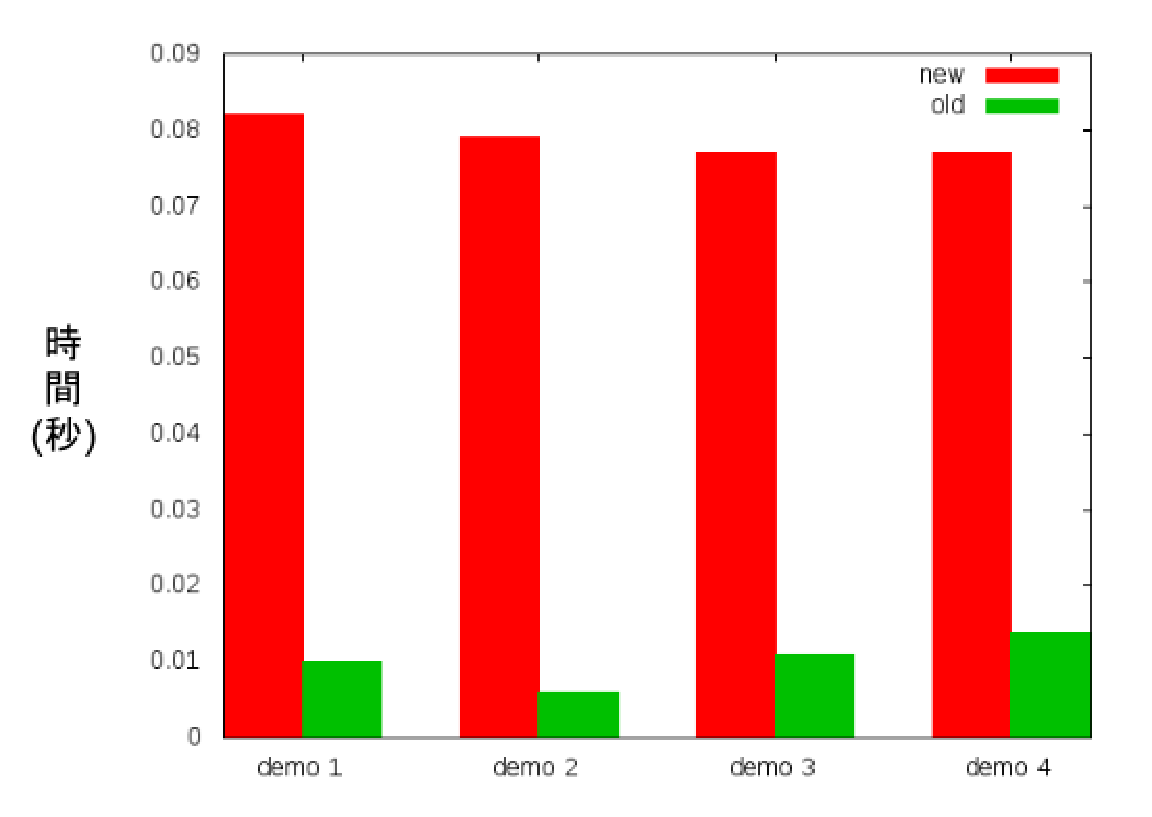
\includegraphics[scale=0.75]{graph.eps}
\caption{コンパイル時間の比較}
\label{graph}
\end{figure}

グラフでは赤色はNodeJSで書かれたコンパイラで、緑はC言語で書かれたコンパイラである。NodeJSで書かれたコンパイラはコンパイル時間が比較的に長いである。それの理由はNodeJSとC言語の速さの差であることが考えられる。新しいコンパイラの方はコンパイル時間の6割ぐらいがEsprimaの構文解析のところで書かれいて、残り4割は命令列生成の処理でかかる時間である。
\FloatBarrier

\section{感想}
実験でコンパイラについていろいろ学習した。特に仮想機械へコンパイルするコンパイラの作り方、働き方について理解した。SSJSVMの命令セットについて理解できたし、古いコンパイラでバグも見つかれたので、TinyJavaScriptプロジェクトにとっても良かったと思う。パーサの探しの段階で、ANTLRについて学習できたし、実はANTLRを使って英語を使う計算機も友達と一緒に開発した。そして、Esprimaについて理解できて、将来Esprimaを使って何かJavaScriptプログラムを書きやすくするパッケージを書こうと思ってます。

\newpage
\begin{thebibliography}{9}
\bibitem{jscompiler}
高田 祥. \textit{ARM 上で動作する JavaScript 処理系の実装}. 電気通信大学 電気通信学部
情報工学科 ソフトウェア学講座. January, 2011.
\bibitem{spidermonkey}
SpiderMonkey 1.6 \newline
http://www-archive.mozilla.org/js/spidermonkey/release-notes/
\bibitem{esprima}
Esprima \newline
http://esprima.org/
\bibitem{esprimaTests}
Esprimaのテスト情報 \\
http://esprima.org/test/ci.html
\bibitem{esprimaGitHub}
Esprimaのソースコード \\
https://github.com/jquery/esprima
\bibitem{ecmascript}
ECMAScript \newline
http://www.ecma-international.org/publications/standards/Ecma-262.htm
\bibitem{antlr}
ANTLR \newline
http://www.antlr.org/
\bibitem{estree}
EStree プロジェクト \\
https://github.com/estree/estree
\end{thebibliography}

\end{document}
